
Ohinata \& Varvarigos (2020) propose a model where the economy is populated by overlapping generations of households that have
a lifespan of two periods: childhood and adulthood. The household’s budget constraint is

    \begin{equation}
    \begin{aligned}
    c_{t} = \omega h_{t} - n_{t}(q+x_{t})
    \end{aligned}
    \end{equation}

where $c_{t}$ denotes consumption and $h_{t}$ is the stock of human capital.Besides, $\omega$ is the wage per unit of effective labour, and  rearing each child entails a fixed cost of $q>0$. Parents spend resources towards the education of each of their offspring using $x_t$ amount.  

Parents can affect each child’s human capital by devoting resources towards their education using $x_t$ units, so the human capital will be determined as : 

    \begin{equation}
    \begin{aligned}
    h_{t+1} = \varphi h_{t}^{\eta} + \psi h_{t}^{\mu}x_t 
    \end{aligned}
    \end{equation}

Where $\phi , \psi > 0$ and $\eta , \mu  \in (0, 1)$. Note that $h_t$ captures intergenerational externalities that generate dynamics in the formation of human capital. The lifetime utility of the household is given by:

    \begin{equation}
    \begin{aligned}
    u_{t} = \gamma \ln(c_t) + (1-\gamma)[\beta \ln(n_t) + \theta \ln(n_t h_{t+1})]
    \end{aligned}
    \end{equation}
    
Households make their choices so as to maximize their lifetime utility in
equation (3), subject to the constraints in equations (1) and (2). The first order condition are :

    \begin{equation}
    \begin{aligned}
    n_t (q+x_t) = \frac{(1-\gamma)(\beta + \theta)}{\gamma + (1-\gamma)(\beta + \theta)} \omega h_t \\
    x_t = \frac{(1-\gamma)\theta}{\gamma + (1-\gamma)(\beta + \theta)}\frac{\omega h_t}{n_t} - \frac{\varphi}{\psi} h_t^{\eta - \mu}
    \end{aligned}
    \end{equation}

The system of equations in (4) can be solved simultaneously to

    \begin{equation}
    \begin{aligned}
    x_t = X(h_t)  = \max \{0, \frac{1}{\beta}[\theta q - (\theta + \beta) \frac{\varphi}{\psi}  h_t^{\eta - \mu}]\}
    \end{aligned}
    \end{equation}
    
and

    \begin{equation}
    \begin{aligned}
    n_t = N(h_t)  = \begin{cases}
                    \frac{(1-\gamma)(\beta + \theta)}{\gamma + (1-\gamma)(\beta + \theta)} \frac{\omega h_t}{q} & \text{if } x_t = 0 \\
                    \frac{(1-\gamma)\beta}{\gamma + (1-\gamma)(\beta + \theta)} \frac{\omega \psi h_t^{1 + \mu - \eta }}{q \psi h_t^{\mu - \eta} - \varphi}   & \text{if } x_t > 0
                     \end{cases}
    \end{aligned}
    \end{equation}
    
A closer look at the result in equation (5) reveals that there are circumstances under which parents might find it optimal not to invest any
resources towards the education of their offspring.The underlying cause for this possibility lies in the fact that, as long as $ \varphi > 0$, each child will still be endowed with units of efficient labour, because of the presence of the intergenerational externality, even though parents might not invest any resources towards their education.\\

\subsection{Dynamics} 

Assumming that  $\mu > \eta $ , when the stock of human capital is relatively low, the utility cost of foregone consumption outweighs the utility
benefit of educating children and increasing their efficiency. Nevertheless, when the stock of human capital is relatively high, its complementary
effect becomes strong enough to guarantee that the return to investment in education is sufficiently high to compensate parents for the utility loss
due to decreased consumption.

\textbf{Lemma 1}: There exist a threshold which comes when the second element of $X$ functions is equalized to zero : 

    \begin{equation}
    \begin{aligned}
    \Tilde{h} \equiv \left[\frac{(\theta + \beta)\varphi}{\theta \psi q}\right]^{\frac{1}{\mu - \eta}}
    \end{aligned}
    \end{equation}

such that 
    \begin{equation}
    \begin{aligned}
    x_t = X(h_t)  = \begin{cases}
                    0 & \text{if } h_t <= \Tilde{h} \\
                     \frac{1}{\beta}\left[\theta q - (\theta + \beta) \frac{\varphi}{\psi}  h_t^{\eta - \mu}\right] & \text{if } h_t > \Tilde{h}
                     \end{cases}
    \end{aligned}
    \end{equation}

We can see that $ X(\Tilde{h}) = 0$ and 

    \begin{equation}
    \begin{aligned}
    X'(h_t) = \frac{(\mu - \eta)(\theta + \beta)\varphi}{\beta\psi}h_{t}^{\eta - \mu-1} > 0
    \end{aligned}
    \end{equation}

The outcome summarized in (7) allows us to combine equations in order to express human capital accumulation as : 
    \begin{equation}
    \begin{aligned}
    h_{t+1} = F(h_t)  = \begin{cases}
                    \varphi h_{t}^{\eta}  & \text{if } h_t <= \Tilde{h} \\
                     \frac{\theta (\psi q h_{t}^{\mu} - \varphi h_{t}^{\eta})}{\beta}  & \text{if } h_t > \Tilde{h}
                     \end{cases}
    \end{aligned}
    \end{equation}

Fertility Dynamics:
We begin the analysis by using the results in equation (6) in order to examine how fertility varies with the stock of human capital.
\textbf{Lemma 2} :
Consider $n_t = N(h_t)$. It is straightforward to establish that (a) when $x_t = 0$ then $N(h_t)>0$ ; (b) when $x_t > 0$ then there exists. 
   
    \begin{equation}
    \begin{aligned}
    \hat{h} \equiv \left[\frac{(1+\mu - \eta)\varphi}{\psi q}\right]^{\frac{1}{\mu - \eta}}
    \end{aligned}
    \end{equation}

such that when $x_t = 0$
    \begin{equation}
    \begin{aligned}
        N'(h_t) = \frac{(1-\gamma)(\beta +  \theta)}{\gamma + (1-\gamma)(\beta + \theta)}\frac{\omega}{q} > 0 
    \end{aligned}
    \end{equation}

but when $x_t > 0$
    \begin{equation}
    \begin{aligned}
        N'(h_t) & = \frac{(1-\gamma)(\beta)}{\gamma + (1-\gamma)(\beta + \theta)q}\omega\psi \\
        & X\left[\frac{(1+\mu + \eta)h_{t}^{\mu - \eta} (q \psi h_{t}^{\mu - \eta} - \varphi) - h_{t}^{1+\mu - \eta}(\mu - \eta)(q \psi h_{t}^{\mu - \eta -1})}{(q \psi h_{t}^{\mu - \eta} - \varphi)^{2}} \right]
    \end{aligned}
    \end{equation}

The sign of the derivative will depend on the sign of the expression inside the square brackets. 

    \begin{equation}
    \begin{aligned}
    N'(h_t) = \begin{cases}
                    < 0     & \text{if } h_t <= \hat{h} \\
                    > 0     & \text{if } h_t > \hat{h}
                     \end{cases}
    \end{aligned}
    \end{equation}

\textbf{Lemma 3}: 
As long as $[(1+\mu - \eta )\theta]/(\theta + \beta)>1$ then $\hat{h} > \Tilde{h}$
Prrof: $\hat{h} > \Tilde{h}$ implies

    \begin{equation}
    \begin{aligned}
    \left[\frac{(1+\mu - \eta)\varphi}{\psi q}\right]^{\frac{1}{\mu - \eta}} >  \left[\frac{(\theta + \beta)\varphi}{\theta \psi q}\right]^{\frac{1}{\mu - \eta}}
    \end{aligned}
    \end{equation}

And this is only true if  $[(1+\mu - \eta )\theta]/(\theta + \beta)>1$ then $\hat{h} > \Tilde{h}$. \\

Therefore, as the stock of human capital grows, the fertility rate increases for $h_t < \tilde{h}$; it declines for $\Tilde{h} < h_t < \hat{h}$; and it increases again for $h_t > \hat{h}$.
Formally,

    \begin{equation}
    \begin{aligned}
    N'(h_t) = \begin{cases}
                    > 0     & \text{if } h_t < \Tilde{h} \\
                    < 0     & \text{if } \Tilde{h} < h_t <= \hat{h} \\
                    > 0     & \text{if } h_t > \hat{h} \\
                    \end{cases}
    \end{aligned}
    \end{equation}
    
Specifically, the fertility rate increases with $h_t$ at relatively low levels of income; it decreases at intermediate levels of income; and it increases again at relatively high levels of income, as the stock of human capital and therefore fertility converge to their long-run (steady-state) values.

Naturally, our objective is to analyse an economy that goes through all the stages of possible demographic changes, as it converges to the longrun equilibrium that is characterized by $h^{*}$.It follows that the subsequent
analysis will focus on a scenario where the steady-state equilibrium lies
above the two thresholds identified previously. \\
\textbf{Lemma 4}: Assume that.

    \begin{equation}
    \begin{aligned}
    q\psi > max \left\{ \left(\frac{\beta}{\theta}\right)^{(\mu - \eta)/(1-\eta)} \frac{(1+\mu -\eta)\varphi^{(1-\mu)/(1-\eta)}}{(\mu - \eta)^{(\mu - \eta)/(1-\eta)}};\frac{(\theta + \beta) \varphi^{(1-\mu)/(1-\eta)}}{\theta} \right\}
    \end{aligned}
    \end{equation}
    
holds. Then $h^{*} > \hat{h}$ \\

\subsection{The full dynamical system} 
The full dynamics of this model are characterized by a non-linear three dimensional system of difference equations.
        \begin{equation}
    \begin{aligned}
    h_{t+1} = F(h_t)  &= \begin{cases}
                    \varphi h_{t}^{\eta}  & \text{if } h_t <= \Tilde{h} \\
                     \frac{\theta (\psi q h_{t}^{\mu} - \varphi h_{t}^{\eta})}{\beta}  & \text{if } h_t > \Tilde{h}
                     \end{cases}\\
    x_t = X(h_t)  &= \max \{0, \frac{1}{\beta}[\theta q - (\theta + \beta) \frac{\varphi}{\psi}  h_t^{\eta - \mu}]\} \\
    n_t = N(h_t)  &= \begin{cases}
                \frac{(1-\gamma)(\beta + \theta)}{\gamma + (1-\gamma)(\beta + \theta)} \frac{\omega h_t}{q} & \text{if } x_t = 0 \\
                \frac{(1-\gamma)\beta}{\gamma + (1-\gamma)(\beta + \theta)} \frac{\omega \psi h_t^{1 + \mu - \eta }}{q \psi h_t^{\mu - \eta} - \varphi}   & \text{if } x_t > 0
                 \end{cases}
    \end{aligned}
    \end{equation}

This line is added to see if overleaf and github fits well. lets see again

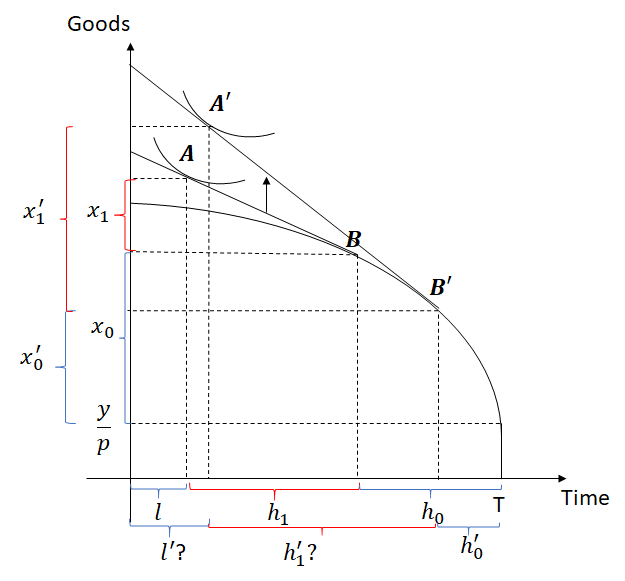
\includegraphics{Images/eitc_poor.png}